% John L. Godlee (johngodlee@gmail.com)

\documentclass[a4paper, 11pt]{article}
%
\usepackage{amsmath}   % Better maths and more symbols
%
\usepackage{siunitx}
%
\usepackage{geometry}  % Set margins
	\geometry{left=2.2cm,
		right=2.2cm,
		top=2.2cm,
		bottom=2cm}
\parskip 0.5cm
\setlength{\parindent}{0.5cm}
%\twocolumn
%
\usepackage{pdflscape} % Allow landscape pages nested in pdf
%
\usepackage{graphics}  % Insert images easily
\usepackage{graphicx}
\graphicspath{ {img/} }
\usepackage{float}  % Fancy graphics placement [H] [H!] arguments
\usepackage{subfig}
%
\usepackage{caption}
%
\usepackage{enumerate}
%
\usepackage{natbib}    % Bibliography management - Use author/date citations
\bibliographystyle{agsmnourl}  % Use my custom agsm bibliography template which never includes URLs in articles
\usepackage{url}
\usepackage{cite}
%
\usepackage{lineno}
\linenumbers
%
\usepackage{eurosym}
\usepackage{textcomp}
\newcommand{\textapprox}{\raisebox{0.5ex}{\texttildelow}}
%
\usepackage{color} 
\newcommand{\todo}[1]{\textcolor{red}{#1}}   % \todo{NOTE TO SELF WRITTEN IN RED}

\title{Changes in forest structure along an elevational gradient in the Peruvian Andes cause species-specific stress responses in tree seedlings}
\author{John L. Godlee}

%--------------------------------------------------------------
\begin{document}
%--------------------------------------------------------------

\maketitle{}

\begin{abstract}
\noindent

\begin{itemize}
\item{We assessed the contribution of biotic competition factors to limiting elevational range shifts of tree species along an Amazon to Andes elevational gradient, focussing on tree seedlings as a key demographic bottleneck for future recruitment.}
\item{Photosynthetic capacity measured using chlorophyll fluorescence estimated photosynthetic stress experienced by naturally occurring seedlings of seven tree species spanning the elevational gradient. Physiognomic plant traits were also measured to assess the degree of local acclimatory response to elevationally dependent environmental factors.}
\item{We used linear mixed effects models to compare the effect sizes of individual biotic competition fixed effects against that of elevation. A matrix of multiple fixed effect mixed effects models were compared statistically to ascertain the best combination of predictors affecting seedling growth and stress metrics.}
\item{}
\end{itemize}

%4 bullet points (1) research conducted + rationale, (2) central methods, (3) key results, (4) main conclusions including key points of discussion. 

\end{abstract}

\section{Introduction}
Rapid anthropogenic climate change is causing many species, across a wide range of taxa, to shift their distributions in space \citep{Chen2011, Hughes2000, Parmesan2006}. The primary forces driving this are an increase in temperature and changes in precipitation regime \citep{Corlett2013, McCain2011}. \citet{Chen2011} estimates that globally, across a range of taxonomic groups, species are experiencing mean latitudinal and altitudinal migration rates of 17.6 $\pm$ 2.9 km and 12.2 $\pm$ 1.8 m per decade, respectively. Previous studies have suggested that the ability of species to respond to changes in mean annual temperature and precipitation regime will be important in determining species success over the coming century \citep{Colwell2008, Chen2011, Feeley2012}. 

Species responses to climate change may occur either in the form of adaptation, \textit{i.e.} changes in phenology, physiology and morphology, or through range shifts over space \citep{Bellard2012}. Range shifts have been observed in many studies across the world, particularly in temperate, sub-arctic and mountainous regions where temperature change is the most extreme \citep{Lenoir2015}. The number of studies documenting adaptational responses are fewer, potentially indicating that climate change is occurring so rapidly as to prevent effective adaptational responses \citep{Mantyka2012}. Range shift rates vary between species depending on their sensitivity to climate and their fecundity, which affects rate of recruitment into newly suitable areas \citep{MacLean2017, Travis2013}. This has the potential to create novel species assemblages as species ranges begin to overlap more or less as they shift, with unknown consequences for ecosystem functionality. Predicting range shifts across space has become an active field of research, (see \citealt{Bellard2012} and references therein), and is being used as a tool to inform conservation strategies to mitigate the effects of climate change on biodiversity and ecosystem functionality \citep{Dawson2011}.

The majority of species distribution models used to predict species range shifts as a conservation tool have used bioclimatic envelopes to constrain species' ranges \citep{Pearson2003, Sinclair2010}. Bioclimatic envelopes are constructed by correlating current species range extent with observed environmental conditions within those boundaries, then projecting spatially explicit climate trends into the future under different climate change scenarios to predict how species range boundaries will adjust in response (e.g. \citealt{Araujo2006, Berry2002, Peterson2002, Thuiller2005}). These models have been criticised often for being overly simplistic, especially when applied at the local scale \citep{McMahon2011}, where other factors that have not been considered by the bioclimatic envelope model become important limiting factors for range shifts. Such factors include unmeasured environmental variables, physical factors such as topography, and biotic interactions with other species \citep{Davis1998, Ettinger2011, Putten2010}. In montane environments, range shifts do not consistently follow an expected upslope trend, with \textapprox{}25\% of species showing a downslope movement and \textapprox{}10\% showing no movement \citep{Lenoir2010}.

When range shifts in a rapidly changing climate are driven by a single environmental variable like mean annual temperature, it is possible that a species will move into an area that is sub-optimal in other ways than those predicted by the model if range shifts outstrip acclimatory/adaptive potential. Range shifts into sub-optimal habitats may lead to reductions in local species abundance and/or richness \citep{Colwell2008}, changes in community composition \citep{Gibson-Reinemer2015}, ecosystem functioning \citep{Bellard2012}, and ecosystem service provision that are not predicted by bioclimatic envelope models \citep{Dobson2011, Isbell2011}. In order to accurately predict range shifts and their consequences for future ecosystem assembly, it is important that predictive range models be expanded to include variables which describe habitat as well as climate \citep{Wisz2013}.

For sessile taxa such as trees, range shifts occur as a result of differential recruitment and mortality over space, at the leading and trailing edges of their range \citep{Corlett2013}. In communities of long-lived tree species however, the forest ecosystem may not shift in equilibrium with the climate as individuals are resilient to gradual changes in climate, developing large root systems and below-ground water and nutrient reserves to buffer against stressful conditions; adult trees may persist where more sensitive seedlings perish \citep{Bell2014, Lenoir2009}. As tree seedlings recruit upslope into areas that are newly suitable in terms of temperature, they will encounter novel biotic environments consisting of canopy trees which first recruited into the area when the climate was different. Forest trees, particularly those in moist tropical forests, often experience high levels of mortality during the seedling recruitment stage, creating a key demographic bottleneck that can impact a species' success, potentially limiting upslope migration \citep{Coomes2000}. Seedling growth is affected by shade regimes created by adult tree canopy gaps. There is abundant evidence that shading from adult tree canopies reduces seedling growth rate and thus increases the probability of seedling mortality, with tropical forest tree seedlings frequently growing into canopy gaps \citep{Valladares2016}. Additionally however, seedlings of many tropical tree species are highly adapted to shade \citep{Matsubara2009}, meaning that if a seedling germinates under an open space in the canopy, especially in the tropics at a higher elevation, where UV-B intensity is higher, mortality by UV-B and heat damage to photosynthetic machinery is quite probable \citep{Krause2001, Li2010}. Many species found at high altitudes have specific adaptations to avoid UV-B damage to photosynthetic machinery, such as vertically stacked palisade mesophyll cells and thick cuticles to reduce UV-B absorption, and generally smaller thicker leaves \citep{Prado2012}. Species found at low altitudes however, are less adapted to high UV-B environments, instead possessing adaptations to make the most of the diminished light levels found under thick tree canopy, particularly during the seedling growth stage. If seedlings germinate in areas that have a different overstorey shade regime and forest structural type to that which they are adapted to grow in, damage may occur leading to loss of photosynthetic capacity, reducing growth rates and occasionally resulting in seedling mortality. 

Montane forest physical structure also varies with elevation. Lowland forests often have lower tree density, with relatively few young trees in the light-deprived understorey, but a higher canopy cover due to adult trees being larger. Plant ground cover is generally greater at higher altitudes, with many epiphytic and ground-level herbaceous species \citep{Martin2010}. Tree seedlings moving upslope may also therefore compete with existing trees and herbaceous flora for nutrients and rootspace, although there is some separation between seedling and adult tree rooting depths for most species \citep{Lewis2000}, especially for the largest trees. These factors acting as limitations to upslope migration of tree species in tropical montane forests may lead to species' ranges narrowing from the bottom up, with increased mortality due to temperature at the bottom of the elevational range, but without increased recruitment at the top end of the elevational range. This seedling mortality bottleneck provides a limiting factor to the success of tropical forest tree species experiencing range shifts and raises concern for their conservation as keystone species of these highly biodiverse ecosystems.

\todo{Talk more about the pecularities and importance of studying the cloud forest elevational gradient}

In this study, along a moist tropical forest elevational gradient in the Peruvian Andes, we investigated the role of biotic effects from existing forest structure on the physiology and physiognomy of tree seedlings across their elevational ranges, in order to increase our knowledge of the dynamics of montane cloud forest tree species elevational range shifts. We tested three hypotheses: 1) Within a species, seedlings growing at higher elevations would experience higher levels of photosynthetic stress than those at lower elevations, 2) Species would differ in their degree of acclimation to variation in adult tree forest structure, and 3) A combination of biotic and abiotic explanatory variables would best explain variation in seedling physiognomic and physiological traits across their elevational range.

\section{Materials and Methods}
\subsection{Study Site}
Data collection was conducted across 10 permanent 1 ha forest plots in the Kos\~{n}ipata Valley of Man\'{u} National Park, Peru (-13\textdegree N, -71\textdegree W, Figure \ref{sites}, Table \ref{site_char}). The Kos\~{n}ipata Valley has been identified as a migration corridor for lowland species to migrate to higher elevations in response to temperature increase \citep{Feeley2011} and so is an appropriate location to study range shift drivers. Plots are situated between 400 and 3200 m.a.s.l. along this migration corridor (Table \ref{site_char}, Figure \ref{ranges}). The plots form part of a larger plot network established by the Andes Biodiversity and Ecosystem Research Group (ABERG) in 2003 \citep{Malhi2010, Girardin2014}, and are located within the Tropical Andes biodiversity hotspot identified in \citet{Myers2000}. The plots used in this study contain 719 tree species, and the valley as a whole contains an estimated 1167 tree species (ABERG unpublished data).

\begin{figure}[H]
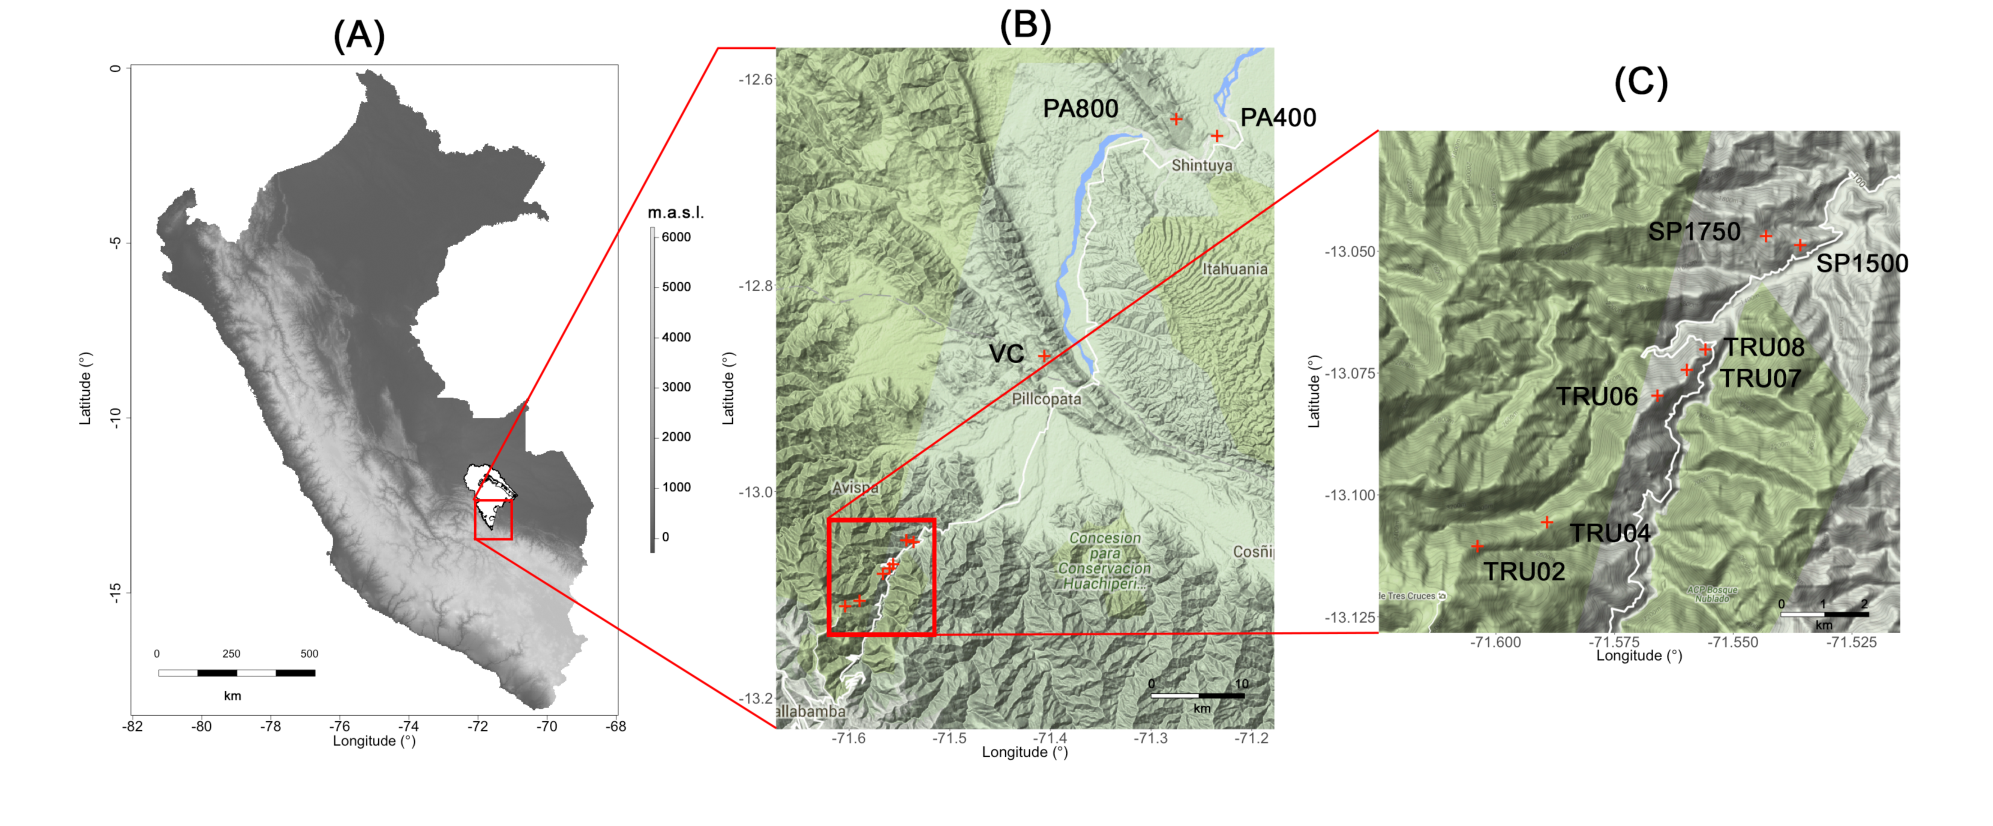
\includegraphics[width=\textwidth]{sites}
\centering
\caption{Maps showing the location of the study area and plot locations. (A) The site location within Peru with elevation shading, showing the proximity to Man\'{u} National Park (white area). (B) The location of the 1 ha plots within the Kos\~{n}ipata Valley. (C) An enlargement of the Trocha Union and San Pedro plot groups. Red crosses indicate plot location, white lines in maps (B) and (C) indicate roads, text labels in (B) and (C) are plot codes, dark green areas in (B) and (C) denote the bounds of Man\'{u} National Park.}
\label{sites}
\end{figure}


% Table created by stargazer v.5.2.2 by Marek Hlavac, Harvard University. E-mail: hlavac at fas.harvard.edu
% Date and time: Mon, Oct 21, 2019 - 19:13:07
\begin{table}[!htbp] \centering 
  \caption{Site environmental characteristics for each 1 ha plot sampled. NA indicates that no data was available. Adapted from \citet{Whitaker2014}.} 
  \label{site_char} 
\begin{tabular}{@{\extracolsep{-2pt}} cccccccc} 
\\[-1.8ex]\hline 
\hline \\[-1.8ex] 
{Site} & {Elev. (m (m))} & {Precip. (mm y\textsuperscript{-1})} & { Mean temp. (\textdegree{}C)} & {Soil C (\%)} & {Soil N (\%)} & {Soil pH} & {Trees ha\textsuperscript{-1}} \\
\hline \\[-1.8ex] 
PA1 & 406 & NA & NA & NA & NA & NA & 475 \\ 
PA2 & 822 & NA & NA & NA & NA & NA & 690 \\ 
VC1 & 861 & 3087 & 20.7 & 16 & 1.4 & 3.8 & 645 \\ 
SP1 & 1497 & 2631 & 17.4 & 10.5 & 1 & 4 & 860 \\ 
SP2 & 1770 & 2631 & 15.8 & 26 & 1.8 & 4.2 & 887 \\ 
TU8 & 1839 & 2472 & 16 & 31 & 2 & 4.3 & 954 \\ 
TU7 & 2135 & 1827 & NA & 37 & 2.1 & 4 & 1060 \\ 
TU6 & 2281 & NA & 14.9 & NA & NA & NA & 1101 \\ 
TU4 & 2733 & 2318 & 11.1 & 28.5 & 1.8 & 3.9 & 1287 \\ 
TU2 & 3213 & NA & 8.9 & 44.5 & 2.6 & 3.8 & 1417 \\ 
\hline \\[-1.8ex] 
\end{tabular} 
\end{table} 


\todo{Add something about the environmental variation within the elevational gradient, presence of cloud zone etc.}

\subsection{Study species} 
We chose seven tree species for comparison from a total of 719 identified species within the 10 study plots. Species were selected according to their contrasting ranges (Figure \ref{ranges}), differences in genus migratory pattern \citep{Feeley2011} (Figure \ref{mig}), and because each species is dominant across it's range in the Kos\~{n}ipata Valley (ABERG, unpublished data) (Figure \ref{rank_abund}). Seedlings of \textit{Myrcia} spp. are difficult to reliably identify to species in the field due to similar morphology and were instead sampled as a composite of three potential species: \textit{Myrcia splendens}, \textit{M. fallax}, and \textit{M. rostrata}, the only \textit{Myrcia} species known to be present in our plots from previous ABERG censuses. They are referred to as \textit{Myrcia spp.} from here onwards. 

% Despite having no quantitative range shift prediction information, \textit{Iriartea deltoidea} and \textit{Dictyocaryum lamarckianum} were included in order to observe potential differences in response between monocot and dicot species, as both are monocots. Both \textit{I. deltoidea} and \textit{D. lamarckianum} are large-seeded palm species, as such, they are expected to be migrating upslope, similar to other large-seeded palms \citep{Hillyer2010}.

\begin{figure}[H]
\includegraphics[width=\textwidth]{ranges}
\centering
\caption{Elevations of study plots for each species (coloured points) with the upper and lower range extents for each species (black squares). Plot elevations are marked as dashed lines and labelled.}
\label{ranges}
\end{figure}


% Table created by stargazer v.5.2.2 by Marek Hlavac, Harvard University. E-mail: hlavac at fas.harvard.edu
% Date and time: Fri, Aug 30, 2019 - 11:24:18
\begin{table}[!htbp] \centering 
  \caption{The sites at which tree seedlings were sampled for each species, with the number of seedlings successfully sampled per site.} 
  \label{species_elevcode_tally} 
\begin{tabular}{@{\extracolsep{5pt}} llr@{\hspace{0.2\tabcolsep}}lr@{\hspace{0.2\tabcolsep}}lr@{\hspace{0.2\tabcolsep}}l} 
\\[-1.8ex]\hline 
\hline \\[-1.8ex] 
{Species code} & {Species} & \multicolumn{2}{c}{Bottom} & \multicolumn{2}{c}{Middle} & \multicolumn{2}{c}{Top} \\
\hline \\[-1.8ex] 
AV & \textit{Alzatea verticillata} & SP1750 & =7 & TRU08 & =5 & TRU07 & =6 \\ 
CR & \textit{Clethra revoluta} & SP1750 & =7 & NA & & TRU04 & =8 \\ 
CT & \textit{Clusia thurifera} & SP1750 & =9 & TRU07 & =9 & NA & \\ 
HG & \textit{Hedyosmum goudotianum} & TRU08 & =10 & TRU04 & =10 & TRU02 & =11 \\ 
MS & \textit{Myrcia} spp. & PA800 & =10 & SP1500 & =8 & TRU07 & =10 \\ 
SP & \textit{Schefflera patula} & TRU08 & =9 & TRU07 & =12 & NA & \\ 
TG & \textit{Tapirira guianensis} & SP1500 & =10 & NA & & TRU08 & =10 \\ 
\hline \\[-1.8ex] 
\end{tabular} 
\end{table} 



\begin{figure}[H]
\includegraphics[width=\textwidth]{rank_abund}
\centering
\caption{Rank abundance curve of all individuals \textgreater{}10 cm DBH of all species found in the plots measured in this study. Census data from 2014 (ABERG, unpublished data). Species sampled as part of this study are highlighted in red. \textit{Myrcia} species which form the composite \textit{Myrcia} spp. are highlighted in green.}
\label{rank_abund}
\end{figure}

\begin{figure}[H]
\includegraphics[width=\textwidth]{mig}
\centering
\caption{Estimated elevational migration rates within the Kos\~{n}ipata valley for selected genera of which species are studied here. Migration rates are estimated using shifts in the centre of gravity of tree basal area as measured in the ABERG 1 Ha plot network.}
\label{mig}
\end{figure}


\subsection{Sampling and Measurement}
Species were sampled in three plots representing the top, middle and bottom elevational extents of their ranges (Figure \ref{ranges}). Within each plot, a maximum of 10 seedlings were sampled. To minimise the chance of pseudo-replication of sampled seedlings, seedlings closer than 10 m to another sampled seedling were excluded from the analysis, as it could not be guaranteed that the stems were not connected by a stolon or rhizome. It also ensured that competition measurements were truly independent. Within a cluster of seedlings within 5 m of each other, each seedling was assigned a number and a random number generator was used to choose a single seedling for measurement.

Proxies for photosynthetic capacity were measured on the highest fully-expanded leaf of each seedling to assess seedling stress. Seedlings under physiological stress may deactivate or lose chlorophyll photo-centres, lowering photosynthetic capacity. Chlorophyll-$\alpha$ fluorescence was measured to estimate photosynthetic capacity using a Walz Mini-PAM II (Walz Effeltrich, Germany), on a randomly selected area of adaxial leaf surface, avoiding prominent leaf veins. These measurements were used to calculate $F_v/F_m$ according to \citet{Genty1989}:

\begin{equation} \label{eq:fvfm}
F_v/F_m = (F_m - F_o)/F_m
\end{equation}

Where $F_m$ is the maximal fluorescence in the dark and $F_o$ is the minimal fluorescence in the dark \citep{Maxwell2000}. Fluorescence measurements were taken after exposing the seedling to 30 minutes of total darkness by covering with an opaque black bag, to ensure complete dark adaptation \citep{Campbell2007}. Dark-adapted $F_v/F_m$ measures the photosynthetic capacity of the leaf by relaxing the photo-centres prior to the fluorescence measurement. $F_v/F_m$ is preferable to other chlorophyll fluorescence measures to estimate underlying physiological stress as it removes the noise created by environmental conditions at the time of measurement, instead providing a measure of the underlying photosynthetic capacity. A reduction in $F_v/F_m$ is indicative of plant stress. Here, individuals with $F_v/F_m$ values \textless{}0.7 are considered to be experiencing stress \citep{Maxwell2000}. 

In addition to $F_v/F_m$, leaf chlorophyll content was measured using a multi-spectral SPAD-meter (Minolta SPAD-502Plus, Spectrum Technologies, Plainfield, Illinois, USA). To account for variation in chlorophyll content across the leaf \citep{Serrano2008}, SPAD measurements were taken at three random points on the leaf. The leaf midvein, other prominent veins, and areas of obvious leaf necrosis were avoided in these measurements. The mean of the SPAD values was used to calculate an estimate leaf chlorophyll content using the conversion factor outlined in \citet{Coste2010} for neotropical broadleaf tree species:

\begin{equation} \label{eq:chl-spad}
Chl_\alpha = 117.1 \times \frac{\overline{SPAD}}{148.84 - \overline{SPAD}}
\end{equation}


\subsection{Leaf and whole-plant morphological measurements}

After leaf physiological measurements, the same upper-most expanded leaf was removed from the seedling and hydrated for a minimum of 48 hours to reverse any leaf curling or contraction in thickness due to dessication. With the petiole removed, each leaf was photographed and the projected lead area was calculated using ImageJ Version 1.51 \citep{Schneider2012}. Mean leaf thickness was calculated using a digital micrometer (0-25 mm, Precision Technologies International, Tamworth, Staffordshire, UL) on three random points on the leaf, avoiding the midvein and prominent leaf veins. To quantify whole-seedling physiognomic characteristics we measured stem width below the lowest set of leaves using the digital micrometer and counted the number of fully expanded leaves (excluding cotyledons). We also measured seedling height from the base of the stem to the tip of the upper-most fully expanded leaf. Stem volume was calculated from stem width and seedling height assuming a cylinder of constant diameter. To account for differences in seedling growth stage and to reduce the number of collinear variables in statistical analyses, stem height and number of leaves was expressed as the ratio of number of leaves per unit stem height.

\subsection{Competition measurements}

To assess adult-seedling competition interactions we used two metrics, Leaf Area Index of canopy foliage, and a metric approximating the degree of crowding from surrounding adult trees. Leaf Area Index (LAI) was calculated from hemispherical photographs of the forest canopy above each seedling. Photographs were captured under uniformly overcast cloud conditions to avoid lens flare and to aid in delineation of foliage from sky during processing \citep{Frazer2001}. Images were taken with a Coolpix 4500 compact camera, with a Nikon FC-E8 hemispherical fisheye converter lens. Images were constrained to a 60\textdegree{} circular azimuthal field of view in order to restrict LAI calculations to the part of the sky where the majority of photosynthetically active radiation penetrates the canopy \citep{Jupp2009, Jonckheere2004}. Images were then converted to 8-bit grayscale and binarized manually in ImageJ 1.51 to separate sky from plant material. Binarized images were then analyzed using Hemiphot \citep{hemiphot} in R to estimate LAI as the projected leaf area per unit ground area (m\textsuperscript{2} m\textsuperscript{-2}).

To approximate crowding from adult trees, we used an adapted version of the Iterative Hegyi Index \citep{Hegyi1974, Lee2004, Seifert2014}. Our adapted `Iterative Seedling Index' ($ISI$) uses adult tree trunk diameter at \textapprox{}1.3 m from ground level (Diameter at Breast Height, DBH) and the distance of trees from the seedling to calculate an index for each seedling. Higher $ISI$ values may result from combinations of  greater adult tree DBH and adult trees being closer to the seedling, higher values indicate greater competition pressure from surrounding adult trees:

\begin{equation}
\label{eq:ISI}
ISI_i = log(\sum_{j=1}^n (\frac{1}{{DIST_i}_j} D_j))
\end{equation}

where $D_j$ is the DBH of a competitor tree and ${{DIST_i}_j}$ is the euclidean distance between seedling $i$ and competitor tree $j$. $ISI$ was log transformed for analysis, as results spanned multiple orders of magnitude. The `iterative' aspect refers to the selection of competitor trees. An iterative selection method for competitive trees assumes that if the path between two trees is blocked by some obstacle, \textit{e.g.} another tree, the intensity of competition between them will be greatly reduced \citep{Gadow1999}. The radius around the seedling is divided into 12 30\textdegree{} sectors, where only the nearest tree \textgreater{}10 cm DBH within each sector is measured (Figure \ref{hegyi}). The size of the competition radius ($C_R$) is defined as:

\begin{equation}
\label{eq:CR}
C_R = 2 \times \sqrt{\frac{10000}{N}}
\end{equation}

where $N$ is the number of trees \textgreater10 cm DBH per ha (stand density). Stand density data was taken from ABERG census data within each plot (ABERG unpublished data) and used to interpolate the value of $C_R$ for plot VC, for which no stand density data exists. We fitted a linear regression between the elevation and trees ha\textsuperscript{-1} of each plot, and interpolated the trees ha\textsuperscript{-1} of plot VC using the regression fit (Figure \ref{comp_radius_fit}). $C_R$ was rounded to the nearest metre for ease of measurement (Table \ref{comp_radius}). 

\begin{figure}[H]
\includegraphics[width=0.5\textwidth]{hegyi}
\centering
\caption{Schematic diagram showing the iterative selection of active competitor trees for the Iterative Seedling Index (ISI) (Equation \ref{eq:ISI}). Trees marked in green (A, B, D) are active competitors for the tree of interest (black diamond). Trees marked in red (C, E, F, G) are non-active competitors, coloured circle radius represents tree DBH. The double circle defines the Competition Radius ($C_R$) (Table \ref{comp_radius}, Equation \ref{eq:CR}). Dashed lines represent 30\textdegree{} zones within which to choose one active competitor. D is the active competitor of its zone as it is the nearest competitor of a suitable DBH (\textgreater{}10 cm). F is not an active competitor as it is \textless{}10 cm DBH. G is not an active competitor as it is outside the competition radius. Adapted from \citet{Lee2004}.}
\label{hegyi}
\end{figure}

\begin{figure}[H]
\includegraphics[width=\textwidth]{comp_radius_fit}
\centering
\caption{Linear regression with 95\% confidence interval of number of trees per hectare for each site, used to estimate number of trees per hectare for site VC. $R^2$ = 0.896, $F_{(1,7)}$ = 579.5, $p$ \textless{} 0.001.}
\label{comp_radius_fit}
\end{figure}


% Table created by stargazer v.5.2.2 by Marek Hlavac, Harvard University. E-mail: hlavac at fas.harvard.edu
% Date and time: Tue, Oct 22, 2019 - 11:48:45
\begin{table}[!htbp] \centering 
  \caption{} 
  \label{comp_radius} 
\begin{tabular}{@{\extracolsep{5pt}} ccc} 
\\[-1.8ex]\hline 
\hline \\[-1.8ex] 
site & trees\_ha & c\_r \\ 
\hline \\[-1.8ex] 
PA2 & $690$ & $8$ \\ 
VC1 & $645$ & $8$ \\ 
SP1 & $860$ & $7$ \\ 
SP2 & $887$ & $7$ \\ 
TU8 & $954$ & $6$ \\ 
TU7 & $1060$ & $6$ \\ 
TU6 & $1101$ & $6$ \\ 
TU4 & $1287$ & $6$ \\ 
TU2 & $1417$ & $5$ \\ 
\hline \\[-1.8ex] 
\end{tabular} 
\end{table} 



\subsection{Statistical Analysis}

A matrix of single predictor linear mixed effects models were compared to test for the presence and strength of the causal relationship between each of the two competition variables and each of the six plant traits. The fixed effect of elevation was also included in this comparison in order to compare the effects of competition to that of other unmeasured elevationally dependent environmental effects. All fixed effects were standardised and rescaled with a mean of 0 and a standard deviation of 1 to allow easy comparison of effect sizes, according to \citep{Grueber2011}. Model comparison was performed on models fitted using Maximum Likelihood (ML) estimates \citep{Bolker2008}. Model quality was compared using Akaike Information Criteria ($AIC$) \citep{Akaike1992}, Akaike weights ($W_i$), and fixed effect marginal pseudo-R\textsuperscript{2} values ($R_M^2$) using \textit{r.squared.GLMM()} from the \textit{MuMIn} package \citep{MuMIn}. Random effects of site and species were added to the models. Site was added as a random intercept effect to account for pseudo-replication in site characteristics within which multiple seedlings per site were sampled. Tree species was added as a random slope effect to account for differences in morphology and physiology between seedlings and to allow for comparison of model slopes between species. As there were multiple species sampled within a single plot, but not all plots contained all species, these models have a partially crossed random effects structure.

The single fixed effect models were compared using $\Delta$AIC\textsubscript{r} against a random effects model to assess whether the fixed effects captured real variation in plant traits. Models were also analysed with an approximation of the variance explained by the model ($R_C^2$) using \textit{r.squared.GLMM()} from the \textit{MuMIn} package \citep{MuMIn}, and slope coefficients (Figure \ref{single_pred_daic}, Figure \ref{single_pred_slope}) to compare their relative effect on plant traits. Single fixed effect model structures were as follows:

\begin{equation}
\label{eq:slope_model}
\todo{Y_{ij} = \beta_{0} + \beta_{1}X_{ij} + u_{0j} + u_{1j}X_{ij} + \epsilon_{ij}}
\end{equation}

\todo{where $Y_{ij}$ is the response variable of species $i$ at site $j$, $X_{ij}$ is the fixed effect value of species $i$ in site $j$. The random intercept grouping effect of site was used in all models to account for pseudo-replication in site characteristics for seedlings sampled along the elevation gradient.}

To better understand the multiplicative effects of competition and other elevationally dependent environmental variables on plant traits we also compared linear mixed effects models with combinations of fixed effects, using $AIC$, $W_i$ and $R_C^2$, to find the model which best explained variation in each plant trait. These models used the same basic model specification as the single fixed effect random intercept models shown above, except with multiple additive fixed effects. To ensure all models converged, these more complicated models only used random intercept effects for species and sites. For initial model comparison, these models were fitted using Maximum Likelihood. All statistical analyses were conducted using R, version 3.2.4 \citep{R2019}. Linear mixed effects models were fitted using the \textit{lme4} package \citep{Bates2015}.

\section{Results}

\subsection{Variation in plant traits across elevation}

All species except \textit{Myrcia} spp. (MS) showed a general positive trend in photosynthetic efficiency ($F_v/F_m$) across their respective elevational ranges, though the spread of $F_v/F_m$ within species was small. Random effect slopes of photosynthetic efficiency over elevation showed that none of the species level regressions dipped below the critical stress threshold of 0.7. Of the 151 measured seedlings, 12 had an $F_v/F_m$ below 0.7. Of those 12 seedlings, 4 were \textit{Alzatea verticillata} (AV), 2 were  \textit{Clethra revoluta} (CR) and 1 each from \textit{Clusia thurifera} (CT) and \textit{Myrcia} spp. (MS) (Figure \ref{traits_elev_slopes}). 

Chlorophyll-$\alpha$ generally decreased with elevation, with negative trends in \textit{A. vertitcillata} (AV), \textit{C. thurifera} (CT), \textit{Myrcia} spp. (MS), \textit{Schefflera patula} (SP) and \textit{Tapirira guianensis} (TG). \textit{C. revoluta} (CR)  and \textit{Hedyosmum goudotianum} (HG) had positive trends (Figure \ref{traits_elev_scatter}). 

The relationship between physiognomic plant traits and elevation varied between species. Leaf:height ratio generally decreased with increasing elevation, with seedlings becoming less leafy with elevation, except for \textit{A. verticillata} (AV) which showed a negative U-shaped relationship, and \textit{H. goudotianum} (HG) which showed a positive hump-shaped relationship (Figure \ref{spaghetti}). Leaf area did not vary meaningfully across elevation except in \textit{S. patula} (SP) where it decreased and \textit{T. guianensis} (TG) where it increased. Leaf thickness generally increased or remained the same with elevation, except in \textit{C. thurifera} (CT), which had a weak negative relationship, with some individuals at the lower end of the elevational range having particularly thick leaves. Stem volume was similarly unaffected by elevation, except in \textit{S. patula} (SP), where it decreased with elevation and in \textit{H. goudotianum} (HG) where it increased, driven by very large seedlings at the top end of the elevation gradient.

Species with restricted elevational ranges were more likely to have steeper relationships of both physiological and physiognomic plant traits across elevation, e.g. \textit{A. verticillata} (AV), \textit{C. thurifera} (CT), \textit{S. patula} (SP) and \textit{T. guianensis} (TG). These species with restricted elevational ranges also inhabit the cloud zone of the forest elevational gradient (Figure \ref{slope_elev_scatter}).

\begin{figure}[H]
\includegraphics[width=\textwidth]{box}
\centering
\caption{Box plots showing the variation in plant trait values within each species.}
\label{box}
\end{figure}

\begin{figure}[H]
\includegraphics[width=\textwidth]{spaghetti}
\centering
\caption{Interaction plots showing the variation in plant trait values within each species.}
\label{spaghetti}
\end{figure}

\begin{figure}[H]
\includegraphics[width=\textwidth]{traits_elev_scatter}
\centering
\caption{Scatter plots with linear model fits for each species, showing the variation in plant stress variables and plant traits across elevation.}
\label{traits_elev_scatter}
\end{figure}

\subsection{Directional effects of adult competition on plant traits}

\begin{figure}[H]
\includegraphics[width=\textwidth]{traits_elev_slopes}
\centering
\caption{Interval plots showing the effect sizes (slopes) of each species in single fixed effect linear mixed effects models of plant traits against elevation variables.}
\label{traits_elev_slopes}
\end{figure}

\begin{figure}[H]
\includegraphics[width=\textwidth]{single_pred_slope}
\centering
\caption{Model slopes for each single fixed effect model of plant traits predicted by elevation and competition variables. Error bars are $\pm$1 standard error. Models where $\delta{}AIC_r$ was less than two and therefore not appreciably better than an equivalent random effects models are shown as asterisks.}
\label{single_pred_slope}
\end{figure}

\begin{figure}[H]
\includegraphics[width=\textwidth]{single_pred_r2m}
\centering
\caption{The approximation of marginal $R^2$ explained by the fixed effect of each single fixed effect model.}
\label{single_pred_r2m}
\end{figure}

\begin{figure}[H]
\includegraphics[width=\textwidth]{slope_elev_scatter}
\centering
\caption{Slopes for each species in a linear model of plant trait vs. elevation, showing variation in model slope with elevational range.}
\label{slope_elev_scatter}
\end{figure}

Across species, models with single fixed effects poorly estimated variation in plant traits. Models with the fixed effect of elevation explained the greatest amount of variation in plant traits, notably stem volume and Chlorophyll-$\alpha$, but neither of these models were appreciably better than a random effects model including only the effects of site and species (Figure \ref{single_pred_r2m}). Models with ISI predicting stem volume and LAI predicting leaf thickness were the only two single fixed effect models using competition variables which provided adequate model fit (Figure \ref{single_pred_r2m}). ISI caused a decrease in stem volume, LAI caused a decrease in leaf thickness.

Table \ref{best_mod_multi_output} shows the fixed effects and model fit measures from the best fitting multiple fixed effect models used to predict plant traits. All of the best multiple predictor mixed effects models included elevation as a fixed effect. All of the best models, except the model predicting leaf Chlorophyll-$\alpha$, included both adult competition predictor variables, ISI and LAI, alongside that of elevation (Figure \ref{multi_pred_slope}). The variance explained by these best multiple predictor mixed effects models was higher than that for the single fixed effects models. $F_v/F_m$, Leaf:height ratio, Stem volume and Leaf thickness had models which were better than a random effects model with $\Delta{}AIC_r > 2$.

In the best fitting multiple fixed effect model for $F_v/F_m$, ISI and LAI had contrasting effects. An increase in ISI led to a decrease in $F_v/F_m$ while an increase in LAI led to an increase in $F_v/F_m$. 

\begin{figure}[H]
\includegraphics[width=\textwidth]{multi_pred_slope}
\centering
\caption{}
\label{multi_pred_slope}
\end{figure}


% Table created by stargazer v.5.2.2 by Marek Hlavac, Harvard University. E-mail: hlavac at fas.harvard.edu
% Date and time: Fri, Aug 30, 2019 - 09:19:47
\begin{table}[!htbp] \centering 
  \caption{} 
  \label{best_mod_multi_output} 
\begin{tabular}{@{\extracolsep{5pt}} lcS[table-format=3.2]S[table-format=3.2]S[table-format=3.2]S[table-format=3.2]} 
\\[-1.8ex]\hline 
\hline \\[-1.8ex] 
{Response} & {Fixed effects} & {$\Delta{}AIC_r$} & {$W_i$} & {$R^2_c$} & {$R^2_m$} \\
\hline \\[-1.8ex] 
$F_v/F_m$ & Elev. + ISI + LAI & -4.82 & 1 & 0.29 & 0.1 \\ 
Chlorophyll-$\alpha$ & LAI & 0.73 & 1 & 0.28 & 0.01 \\ 
Leaf:height ratio & Elev. + ISI + LAI & -4.31 & 1 & 0.37 & 0.1 \\ 
Leaf area\_log & Elev. + ISI + LAI & -0.06 & 1 & 0.31 & 0.05 \\ 
Stem vol. & Elev. + ISI + LAI & -11.6 & 1 & 0.57 & 0.23 \\ 
Leaf thickness & Elev. + ISI + LAI & -12.59 & 1 & 0.78 & 0.08 \\ 
\hline \\[-1.8ex] 
\end{tabular} 
\end{table} 


\section*{Discussion}

This study aimed to (a) determine whether tree seedling physiological and physiognomic plant traits were affected by competition from adult trees across an elevation gradient, (b) assess how the effects of competition compared to that of elevation, and (c) assess the degree to which plant trait-elevation relationships vary among species. It was found that adult competition variables never influence a given plant trait more than elevation, but that combinations of elevation and competition variables better predict variation in plant traits than elevation alone. Tree species with more restricted elevational ranges, which inhabit the cloud zone of the elevational gradient appear to be more sensitive to variation in biotic environmental factors. Interestingly however, according to $F_v/F_m$ chlorophyll fluorescence measurements, seedlings did not experience greater physiological stress at higher elevations, instead all species exhibited model slopes \textgreater{}0 or approaching 0.

\subsection{Species specific responses to elevation dependent environmental variation}

\subsection{Photosynthetic efficiency ($F_v/F_m$)}

\subsection{Limits to future upslope migration}

\subsection{Species rarity}

Nine tree species were selected for this study. Although these species are common in the areas we sampled (Appendix VI), there are many other species which may react more or less to the biotic environment. There is evidence that rare species are more affected by environmental factors \citep{Lyons2005,Mouillot2013}. Rare species are more likely to occupy specialist niches, which are narrower on a local geographical scale than those of generalist species \citep{Boulangeat2012}. The evolutionary histories of specialists means they are less likely to be able to acclimate to novel environments. Compared to the common species studied here, rare species will not have such a large direct effect on globally significant ecosystem services such as carbon sequestration, albedo, and drainage. This does not mean that rare species do not have the potential to heavily influence ecosystem services indirectly. \citet{Lyons2001}, and \citet{Lyons2005} found that less common species play vital supporting roles in maintaining ecosystem functions such as enhancing invasion resistance and making limiting resources available to other species. 

\subsection{Future studies}

On the basis of this study, which shows that adult-seedling competition intensity varies across elevation and that this variation forms part of the observed plant trait response to elevation, it is recommended that future studies aim to identify competition intensity thresholds beyond which individuals cannot acclimate to the environmental conditions. The location of thresholds should be confirmed using experimental transplantation of seedlings to different elevations to observe variation in plant traits.

In order to determine whether changes in competition intensity also affect adult trees, and thus recruitment, similar studies should be performed on adult trees. This would help to improve the accuracy of species range-shift models by adding the potential variation found within populations and allowing demographically explicit models.
\section*{Conclusion}

\bibliography{elev}

%--------------------------------------------------------------
\end{document}
%--------------------------------------------------------------
